% vim: set spell spelllang=en tw=100 et sw=4 sts=4 foldmethod=marker foldmarker={{{,}}} :

\documentclass[aspectratio=169,compress,10pt]{beamer}

\usepackage{tikz}
\usepackage{xcolor}
\usepackage{complexity}
\usepackage{hyperref}
\usepackage{microtype}
\usepackage{amsmath}                   % \operatorname
\usepackage{amsfonts}                  % \mathcal
\usepackage{amssymb}                   % \nexists
\usepackage[vlined]{algorithm2e} % algorithms
\usepackage{centernot}
\usepackage{listings}
\usepackage{csquotes}
\usepackage{fancyvrb}
\usepackage{bussproofs}
\usepackage{multicol}
\usepackage{booktabs}
\usepackage{mathtools}
\usepackage{pifont}
\usepackage{marvosym}
\usepackage{cancel}

\usepackage{holtexbasic}
\usepackage{environ}
\NewEnviron{holthmenv}{%
  \scalebox{1.0}{\begin{array}[t]{l}
  \BODY
  \end{array}}}
\newcommand{\us}{\_}
\renewcommand{\HOLTokenTurnstile}{\ensuremath{\vdash\!\!}}
\renewcommand{\HOLConst}[1]{\textsf{\small #1}}
\renewcommand{\HOLFieldName}[1]{\textsf{\small #1}}
\renewcommand{\HOLSymConst}[1]{\HOLConst{#1}}
\renewcommand{\HOLTyOp}[1]{\HOLConst{#1}}
\renewcommand{\HOLinline}[1]{\textsf{\ensuremath{#1}}}
\renewcommand{\HOLKeyword}[1]{\ensuremath{\mathsf{#1}}}
\renewcommand{\HOLTokenBar}{\ensuremath{\mathtt{|}}}
\renewcommand{\HOLTokenLeftrec}{\ensuremath{\langle\!|}}
\renewcommand{\HOLTokenRightrec}{\ensuremath{|\!\rangle}}
\renewcommand{\HOLTokenLsl}{\raisebox{.15em}{\ensuremath{}\scriptsize{\textless\rule{-0.1em}{0em}\textless}{}}}

\renewcommand{\HOLStringLitDG}[1]{\scalebox{0.9}{\texttt{"#1"}}}
\renewcommand{\HOLStringLit}[1]{\scalebox{0.9}{\texttt{"#1"}}}
\renewcommand{\HOLCharLit}[1]{\scalebox{0.9}{\#\texttt{"#1"}}}
\newcommand{\HOLcount}[1]{\HOLTokenLeftbrace{}\HOLConst{0}\HOLSymConst{,}\HOLConst{1}\HOLSymConst{,}\HOLConst{...}\HOLSymConst{,}#1\HOLSymConst{\ensuremath{-}}\HOLConst{1}\HOLTokenRightbrace{}}

\usefonttheme{professionalfonts}

\usetikzlibrary{shapes, arrows, shadows, calc, positioning, fit}
\usetikzlibrary{decorations.pathreplacing, decorations.pathmorphing, shapes.misc}
\usetikzlibrary{tikzmark, backgrounds}
\usetikzlibrary{trees, overlay-beamer-styles}
\usetikzlibrary{backgrounds, scopes, graphs, graphs.standard, shapes.geometric}
\usetikzlibrary{shapes.multipart, arrows, arrows.meta, decorations, decorations.markings}

\tikzset{processarrow/.style={->, very thick, decorate, decoration={snake, post length=0.5mm}}}
\tikzset{brace/.style={decorate, decoration={brace}, very thick}}

\definecolor{uofguniversityblue}{rgb}{0, 0.219608, 0.396078}
\definecolor{uofgheather}{rgb}{0.356863, 0.32549, 0.490196}
\definecolor{uofgaquamarine}{rgb}{0.603922, 0.72549, 0.678431}
\definecolor{uofgslate}{rgb}{0.309804, 0.34902, 0.380392}
\definecolor{uofgrose}{rgb}{0.823529, 0.470588, 0.709804}
\definecolor{uofgmocha}{rgb}{0.709804, 0.564706, 0.47451}
\definecolor{uofgsandstone}{rgb}{0.321569, 0.278431, 0.231373}
\definecolor{uofgforest}{rgb}{0, 0.2, 0.129412}
\definecolor{uofglawn}{rgb}{0.517647, 0.741176, 0}
\definecolor{uofgcobalt}{rgb}{0, 0.615686, 0.92549}
\definecolor{uofgturquoise}{rgb}{0, 0.709804, 0.819608}
\definecolor{uofgsunshine}{rgb}{1.0, 0.862745, 0.211765}
\definecolor{uofgpumpkin}{rgb}{1.0, 0.72549, 0.282353}
\definecolor{uofgthistle}{rgb}{0.584314, 0.070588, 0.447059}
\definecolor{uofgrust}{rgb}{0.603922, 0.227451, 0.023529}
\definecolor{uofgburgundy}{rgb}{0.490196, 0.133333, 0.223529}
\definecolor{uofgpillarbox}{rgb}{0.701961, 0.047059, 0}
\definecolor{uofglavendar}{rgb}{0.356863, 0.301961, 0.580392}
\definecolor{uofgleaf}{rgb}{0, 0.517647, 0.239216}

% {{{ theme things
\useoutertheme[footline=authortitle]{miniframes}
\useinnertheme{rectangles}

\setbeamerfont{block title}{size={}}
\setbeamerfont{title}{size=\large,series=\bfseries}
\setbeamerfont{section title}{size=\large,series=\mdseries}
\setbeamerfont{author}{size=\normalsize,series=\mdseries}
\setbeamercolor*{structure}{fg=uofguniversityblue}
\setbeamercolor*{palette primary}{use=structure,fg=black,bg=white}
\setbeamercolor*{palette secondary}{use=structure,fg=white,bg=uofgcobalt}
\setbeamercolor*{palette tertiary}{use=structure,fg=white,bg=uofguniversityblue}
\setbeamercolor*{palette quaternary}{fg=white,bg=black}
\setbeamercolor{block body}{bg=structure!10}
\setbeamercolor{block title}{bg=structure,fg=white}
\setbeamertemplate{blocks}[rounded]
\setbeamercolor*{titlelike}{parent=palette primary}

\beamertemplatenavigationsymbolsempty
\setbeamersize{text margin left=0.5cm}
\setbeamersize{text margin right=0.5cm}

\setbeamertemplate{title page}
{
    \begin{tikzpicture}[remember picture, overlay]
        \node at (current page.north west) {
            \begin{tikzpicture}[remember picture, overlay]
                \fill [fill=uofguniversityblue, anchor=north west] (0, 0) rectangle (\paperwidth, -2.6cm);
            \end{tikzpicture}
        };

        \node (logo) [anchor=north east, shift={(-0.8cm,-0.2cm)}] at (current page.north east) {
            
\includegraphics[keepaspectratio=true,scale=0.5]{../../images/UoG_keyline.pdf}
        };

        \node (logo2) [anchor=north, below=0.2cm of logo.south] {
            
\includegraphics[keepaspectratio=true,scale=0.1]{../../images/RAEngWhite.pdf}
        };

        \coordinate (logos) at ($(logo.south)!0.5!(logo2.north)$);

        \node [anchor=west, xshift=0.8cm] at (current page.west |- logos) {
            \begin{minipage}{0.65\paperwidth}\raggedright
                {\usebeamerfont{title}\usebeamercolor[white]{}\inserttitle}\\[0.2cm]
                {\usebeamerfont{author}\usebeamercolor[white]{}\insertauthor}
            \end{minipage}
        };
    \end{tikzpicture}
}

\setbeamertemplate{section page}
{
    \begin{centering}
        \begin{beamercolorbox}[sep=12pt,center]{part title}
            \usebeamerfont{section title}\insertsection\par
        \end{beamercolorbox}
    \end{centering}
}

\newcommand{\frameofframes}{/}
\newcommand{\setframeofframes}[1]{\renewcommand{\frameofframes}{#1}}

\makeatletter
\setbeamertemplate{footline}
{%
    \begin{beamercolorbox}[colsep=1.5pt]{upper separation line foot}
    \end{beamercolorbox}
    \begin{beamercolorbox}[ht=2.5ex,dp=1.125ex,%
        leftskip=.3cm,rightskip=.3cm plus1fil]{title in head/foot}%
        {\usebeamerfont{title in head/foot}\insertshorttitle}%
        \hspace{0.22\textwidth}%
        {\usebeamerfont{author in head/foot}\insertshortauthor}%
        \hfill%
        {\usebeamerfont{frame number}\usebeamercolor[fg]{frame number}\insertframenumber~\frameofframes~\inserttotalframenumber}
    \end{beamercolorbox}%
    \begin{beamercolorbox}[colsep=1.5pt]{lower separation line foot}
    \end{beamercolorbox}
}

\makeatletter
\setbeamertemplate{mini frame}
{%
  \begin{pgfpicture}{0pt}{0pt}{.04cm}{.04cm}
    \pgfpathcircle{\pgfpoint{0.04cm}{0.04cm}}{0.04cm}
    \pgfusepath{fill,stroke}
  \end{pgfpicture}%
}
\setbeamertemplate{mini frame in current subsection}
{%
  \begin{pgfpicture}{0pt}{0pt}{.04cm}{.04cm}
    \pgfpathcircle{\pgfpoint{0.04cm}{0.04cm}}{0.04cm}
    \pgfsetfillcolor{section in head/foot.bg}
    \pgfusepath{fill,stroke}
  \end{pgfpicture}%
}

\setbeamersize{mini frame size=0.10cm, mini frame offset=0.06cm}
\makeatother

\makeatletter
\newenvironment{nearlyplainframe}[2][]{
    \def\beamer@entrycode{\vspace*{-\headheight}\vspace*{3pt}}
    \setbeamertemplate{headline}
    {%
        \begin{beamercolorbox}[colsep=1.5pt]{upper separation line head}
        \end{beamercolorbox}
        \begin{beamercolorbox}[ht=0.5ex,dp=0.125ex,%
            leftskip=.3cm,rightskip=.3cm plus1fil]{title in head/foot}%
        \end{beamercolorbox}%
        \begin{beamercolorbox}[ht=0.5ex,dp=0.125ex,%
            leftskip=.3cm,rightskip=.3cm plus1fil]{author in head/foot}%
        \end{beamercolorbox}%
        \begin{beamercolorbox}[colsep=1.5pt]{lower separation line head}
        \end{beamercolorbox}
        \vspace*{\headheight}
    }

    \setbeamertemplate{footline}
    {%
        \begin{beamercolorbox}[colsep=1.5pt]{upper separation line foot}
        \end{beamercolorbox}
        \begin{beamercolorbox}[ht=0.5ex,dp=0.125ex,%
            leftskip=.3cm,rightskip=.3cm plus1fil]{author in head/foot}%
        \end{beamercolorbox}%
        \begin{beamercolorbox}[ht=0.5ex,dp=0.125ex,%
            leftskip=.3cm,rightskip=.3cm plus1fil]{title in head/foot}%
        \end{beamercolorbox}%
        \begin{beamercolorbox}[colsep=1.5pt]{lower separation line foot}
        \end{beamercolorbox}
    }

    \begin{frame}[#1]{#2}
    }{
    \end{frame}
}
\makeatother

% }}}

\tikzstyle{state} = [inner sep=1pt]
\tikzstyle{infeasible} = [color=uofgpillarbox]
\tikzstyle{dominated} = [color=uofgcobalt]
\tikzstyle{backwards} = []
\tikzstyle{accept} = [solid, thick]
\tikzstyle{reject} = [dotted, thick]
\tikzstyle{forced} = [color=uofglawn]
\tikzstyle{domination} = [dashed, thick, ->, color=uofgcobalt]

\newcommand{\set}[1]{\{ #1 \}}
\newcommand{\setsize}[1]{{\left|#1\right|}}

\newcommand{\solvernameformat}[1]{\textit{#1}}
\newcommand{\toolformat}[1]{\textit{#1}}
\newcommand{\proofsystemformat}[1]{\textsc{#1}\@}

\newcommand{\veripb}{\toolformat{VeriPB}\xspace}
\renewcommand{\veripb}{\proofsystemformat{VeriPB}\xspace}
\newcommand\veripbid[1]{\alertred{#1}}
\newcommand\veripbConstraint[1]{\alertblue{#1}}

\newcommand{\neighbourhood}{\operatorname{N}}
\newcommand{\vertexset}{\operatorname{V}}
\newcommand{\degree}{\operatorname{deg}}

\providecommand{\reifvar}{r}
\providecommand{\reifimpllft}{\Leftarrow}
\providecommand{\reifimplrt}{\Rightarrow}
\providecommand{\reifequiv}{\Leftrightarrow}
\providecommand{\reifconstrlft}[2]{#1 \reifimpllft #2}
\providecommand{\reifconstrrt}[2]{#1 \reifimplrt #2}
\providecommand{\reifconstrequiv}[2]{#1 \reifequiv #2}

\newcommand{\colorblue}[1]{\textcolor{uofgcobalt}{#1}}
\newcommand{\colorred}[1]{\textcolor{uofgthistle}{#1}}
\newcommand{\colorgreen}[1]{\textcolor{uofglawn}{#1}}

% For highlighting in examples
%   \newcommand<>{\alertred}[1]{{\color#2{red}#1}}
\newcommand<>{\alertred}[1]{{\color#2{uofgthistle}#1}}
\renewcommand<>{\alert}[1]{{\color#2{uofgthistle}#1}}
%   \newcommand<>{\alertblue}[1]{{\color#2[rgb]{0,0,0.7}#1}}
\newcommand<>{\alertblue}[1]{{\color#2{uofgcobalt}#1}}
%   \newcommand<>{\alertgreen}[1]{{\color#2[rgb]{0,0.6,0}#1}}
\newcommand<>{\alertgreen}[1]{{\color#2{uofglawn}#1}}

%%% Extra alert command colours
\newcommand<>{\alertlav}[1]{{\color#2{uofglavendar}#1}}
% Pillarbox is kind of red
\newcommand<>{\alertpillarbox}[1]{{\color#2{uofgpillarbox}#1}}
% Pumpkin is kind of orange
\newcommand<>{\alertpumpkin}[1]{{\color#2{uofgpumpkin}#1}}
\newcommand<>{\alertorange}[1]{{\color#2{uofgpumpkin}#1}}

%%% White text to reserve right amount of space
\newcommand<>{\alertwhite}[1]{{\color#2{white}#1}}

\author{Ciaran McCreesh}
\title{Proof Logging and Symmetry Breaking Constraints}

\begin{document}

{
    \usebackgroundtemplate{
        \tikz[overlay, remember picture]
        \node[at=(current page.south), anchor=south, inner sep=0pt, yshift=-1.4cm]{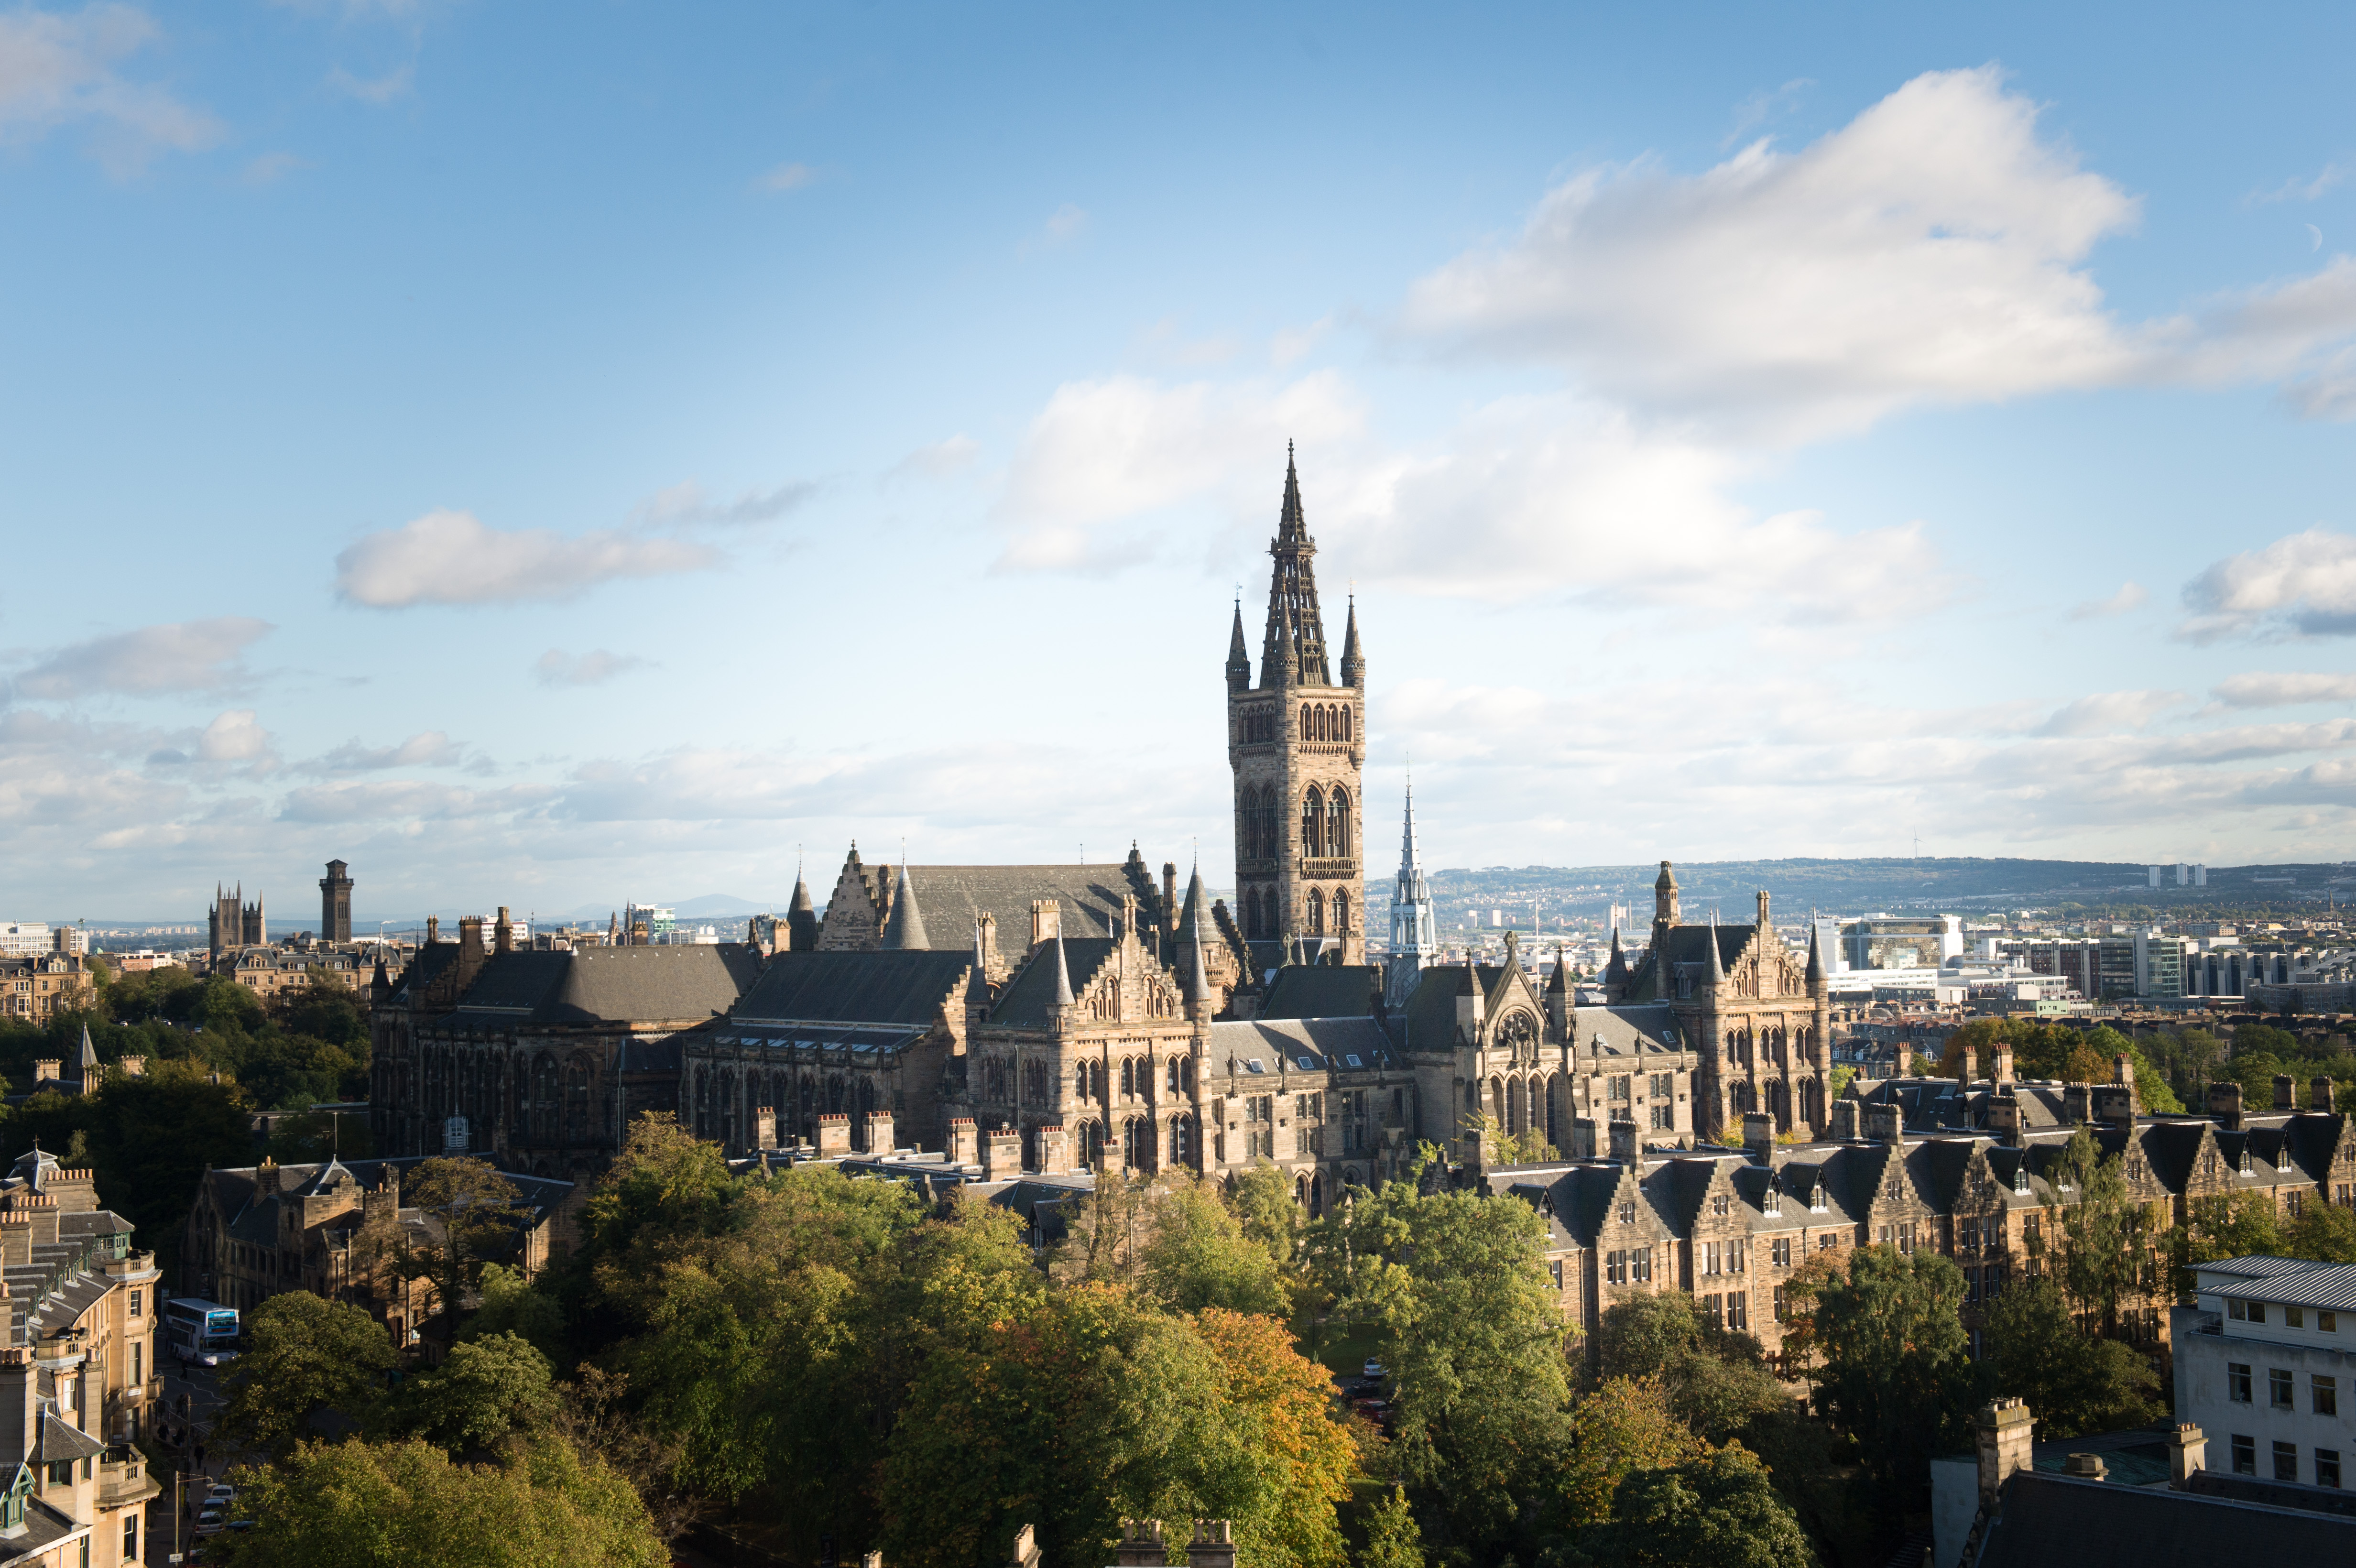
\includegraphics[keepaspectratio=true, width=\paperwidth]{../../images/background.jpg}};
    }
    \begin{frame}[plain,noframenumbering]
        \titlepage
    \end{frame}
}

\section{Constraint Programming}

\begin{frame}{Constraint Programming}
    \begin{itemize}
        \item A declarative way of specifying hard problems.
        \item \textbf{Variables} have \textbf{domains} of possible \textbf{values}.
            \begin{itemize}
                \item Typically, finite subsets of the integers.
            \end{itemize}
        \item \textbf{Constraints} specify restrictions on what values variables can take.
            \begin{itemize}
                \item Lots of different types.
            \end{itemize}
        \item Find a way of giving each variable a value from its domain, respecting all
            constraints.
            \begin{itemize}
                \item Or find the best way of doing so, maximising an objective variable.
            \end{itemize}
    \end{itemize}
\end{frame}

\begin{frame}{The Most Famous Constraint Satisfaction Problem}
    \begin{center}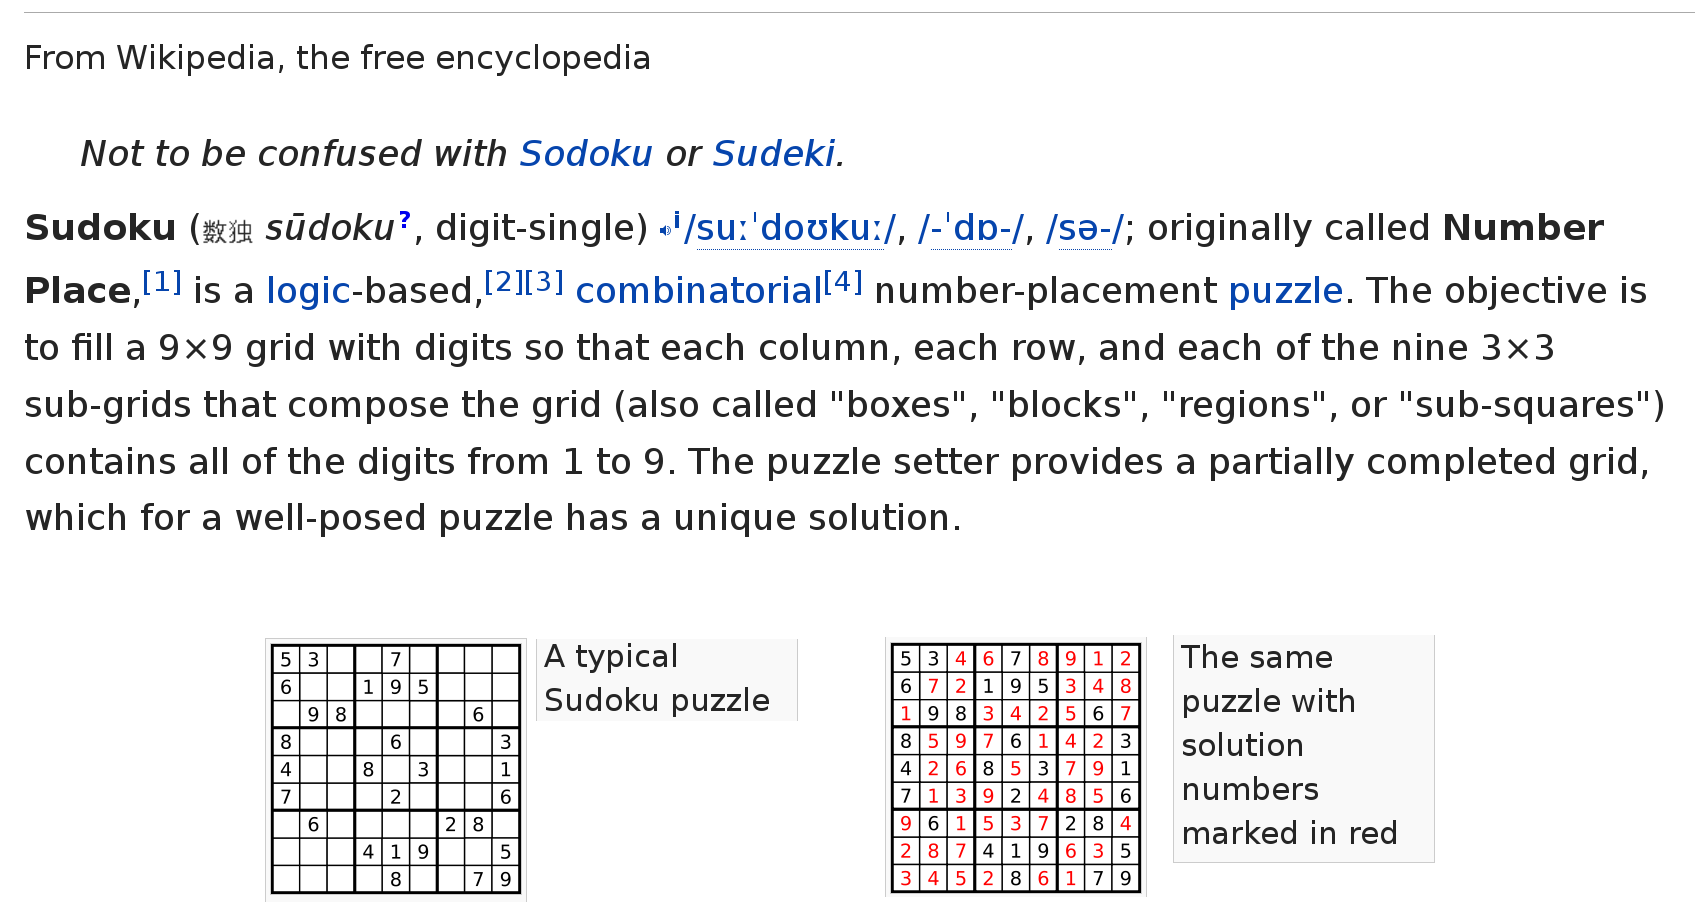
\includegraphics[scale=0.18]{sudoku.png}\end{center}
\end{frame}

\newcommand{\truck}[1]{
    \begin{tikzpicture}[scale=0.5, inner sep=0pt, outer sep=0pt]
        \path[fill=uofgsandstone] (0.9525, -0.7144).. controls (0.9525, -0.7728) and (0.9051, -0.8202) .. (0.8467, -0.8202) -- (0.1058, -0.8202).. controls (0.0474, -0.8202) and (0.0, -0.7728) .. (0.0, -0.7144) -- (0.0, -0.635).. controls (0.0, -0.5766) and (0.0474, -0.5292) .. (0.1058, -0.5292) -- (0.8467, -0.5292).. controls (0.9051, -0.5292) and (0.9525, -0.5766) .. (0.9525, -0.635) -- (0.9525, -0.7144) -- cycle;
        \path[fill=uofgsandstone!60!white] (0.5027, -0.344) -- (0.4768, -0.3175) -- (0.1891, -0.3175).. controls (0.1058, -0.3175) and (0.0794, -0.3704) .. (0.0794, -0.3704) -- (0.0, -0.5281) -- (0.0, -0.6615) -- (0.5027, -0.6615) -- (0.5027, -0.344) -- cycle;
        \path[fill=uofgsandstone!40!white] (0.2381, -0.5292) -- (0.0529, -0.5292) -- (0.1058, -0.4233) -- (0.2381, -0.3704) -- (0.2381, -0.5292) -- cycle;
        \path[fill=uofgsandstone!40!white] (0.2381, -0.8202) circle (0.1058cm);
        \path[fill=black] (0.2381, -0.8202) circle (0.0529cm);
        \path[fill=uofgsandstone!40!white] (0.7144, -0.8202) circle (0.1058cm);
        \path[fill=black] (0.7144, -0.8202) circle (0.0529cm);
        \path[fill=#1] (0.8467, -0.2117) -- (0.4498, -0.2117).. controls (0.3913, -0.2117) and (0.344, -0.2591) .. (0.344, -0.3175) -- (0.344, -0.6615) -- (0.9525, -0.6615) -- (0.9525, -0.3175).. controls (0.9525, -0.2591) and (0.9051, -0.2117) .. (0.8467, -0.2117) -- cycle;
    \end{tikzpicture}
}

\newcommand{\parcel}{
\includegraphics[width=1.2em]{../../2024/a1-poster/parcel.pdf}\,}
\newcommand{\trashpanda}{
\includegraphics[width=1.2em]{../../2024/a1-poster/trashpanda.pdf}\,}
\newcommand{\bed}{
\includegraphics[width=1.2em]{../../2024/a1-poster/bed.pdf}\,}
\newcommand{\chair}{
\includegraphics[width=1.2em]{../../2024/a1-poster/chair.pdf}\,}
\newcommand{\tree}{
\includegraphics[width=1.2em]{../../2024/a1-poster/tree.pdf}\,}
\newcommand{\present}{
\includegraphics[width=1.2em]{../../2024/a1-poster/present.pdf}\,}
\newcommand{\laptop}{
\includegraphics[width=1.2em]{../../2024/a1-poster/laptop.pdf}\,}
\newcommand{\drivera}{
\includegraphics[width=1.2em]{../../2024/a1-poster/driver1.pdf}\,}
\newcommand{\driverb}{
\includegraphics[width=1.2em]{../../2024/a1-poster/driver2.pdf}\,}

\begin{frame}{Industrial Applications}
    \begin{center}
    \begin{minipage}{8cm}
        \centering
        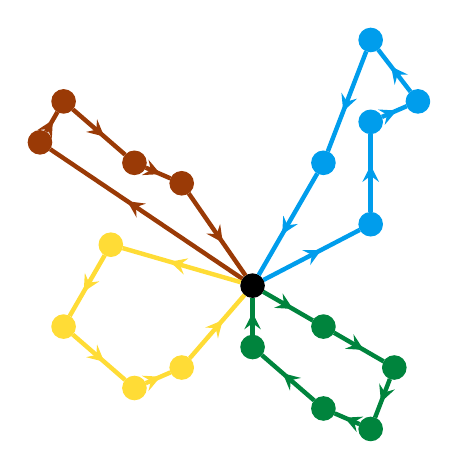
\begin{tikzpicture}
        \begin{scope}[yscale=2.6, xscale=3.0]
        \node (depot) [inner sep=3pt, draw, fill, circle] at (0,0) {};

        \node (RC1) [inner sep=3pt, draw, fill, circle, color=uofgcobalt] at (0.5,0.3) {};
        \node (RC2) [inner sep=3pt, draw, fill, circle, color=uofgcobalt] at (0.5,0.8) {};
        \node (RC3) [inner sep=3pt, draw, fill, circle, color=uofgcobalt] at (0.7,0.9) {};
        \node (RC4) [inner sep=3pt, draw, fill, circle, color=uofgcobalt] at (0.5,1.2) {};
        \node (RC5) [inner sep=3pt, draw, fill, circle, color=uofgcobalt] at (0.3,0.6) {};

        \begin{scope}[decoration={markings, mark=at position 0.6 with {\arrow{stealth}}}]
            \draw [postaction={decorate}, ultra thick, color=uofgcobalt] (depot) -- (RC1);
            \draw [postaction={decorate}, ultra thick, color=uofgcobalt] (RC1)   -- (RC2);
            \draw [postaction={decorate}, ultra thick, color=uofgcobalt] (RC2)   -- (RC3);
            \draw [postaction={decorate}, ultra thick, color=uofgcobalt] (RC3)   -- (RC4);
            \draw [postaction={decorate}, ultra thick, color=uofgcobalt] (RC4)   -- (RC5);
            \draw [postaction={decorate}, ultra thick, color=uofgcobalt] (RC5)   -- (depot);
        \end{scope}

        \node (RR1) [inner sep=3pt, draw, fill, circle, color=uofgrust] at (-0.9,0.7) {};
        \node (RR2) [inner sep=3pt, draw, fill, circle, color=uofgrust] at (-0.8,0.9) {};
        \node (RR3) [inner sep=3pt, draw, fill, circle, color=uofgrust] at (-0.5,0.6) {};
        \node (RR4) [inner sep=3pt, draw, fill, circle, color=uofgrust] at (-0.3,0.5) {};

        \begin{scope}[decoration={markings, mark=at position 0.6 with {\arrow{stealth}}}]
            \draw [postaction={decorate}, ultra thick, color=uofgrust] (depot) -- (RR1);
            \draw [postaction={decorate}, ultra thick, color=uofgrust] (RR1)   -- (RR2);
            \draw [postaction={decorate}, ultra thick, color=uofgrust] (RR2)   -- (RR3);
            \draw [postaction={decorate}, ultra thick, color=uofgrust] (RR3)   -- (RR4);
            \draw [postaction={decorate}, ultra thick, color=uofgrust] (RR4)   -- (depot);
        \end{scope}

        \node (RS1) [inner sep=3pt, draw, fill, circle, color=uofgsunshine] at (-0.6,0.2) {};
        \node (RS2) [inner sep=3pt, draw, fill, circle, color=uofgsunshine] at (-0.8,-0.2) {};
        \node (RS3) [inner sep=3pt, draw, fill, circle, color=uofgsunshine] at (-0.5,-0.5) {};
        \node (RS4) [inner sep=3pt, draw, fill, circle, color=uofgsunshine] at (-0.3,-0.4) {};

        \begin{scope}[decoration={markings, mark=at position 0.6 with {\arrow{stealth}}}]
            \draw [postaction={decorate}, ultra thick, color=uofgsunshine] (depot) -- (RS1);
            \draw [postaction={decorate}, ultra thick, color=uofgsunshine] (RS1)   -- (RS2);
            \draw [postaction={decorate}, ultra thick, color=uofgsunshine] (RS2)   -- (RS3);
            \draw [postaction={decorate}, ultra thick, color=uofgsunshine] (RS3)   -- (RS4);
            \draw [postaction={decorate}, ultra thick, color=uofgsunshine] (RS4)   -- (depot);
        \end{scope}

        \node (RL1) [inner sep=3pt, draw, fill, circle, color=uofgleaf] at (0.3,-0.2) {};
        \node (RL2) [inner sep=3pt, draw, fill, circle, color=uofgleaf] at (0.6,-0.4) {};
        \node (RL3) [inner sep=3pt, draw, fill, circle, color=uofgleaf] at (0.5,-0.7) {};
        \node (RL4) [inner sep=3pt, draw, fill, circle, color=uofgleaf] at (0.3,-0.6) {};
        \node (RL5) [inner sep=3pt, draw, fill, circle, color=uofgleaf] at (0,-0.3) {};

        \begin{scope}[decoration={markings, mark=at position 0.6 with {\arrow{stealth}}}]
            \draw [postaction={decorate}, ultra thick, color=uofgleaf] (depot) -- (RL1);
            \draw [postaction={decorate}, ultra thick, color=uofgleaf] (RL1)   -- (RL2);
            \draw [postaction={decorate}, ultra thick, color=uofgleaf] (RL2)   -- (RL3);
            \draw [postaction={decorate}, ultra thick, color=uofgleaf] (RL3)   -- (RL4);
            \draw [postaction={decorate}, ultra thick, color=uofgleaf] (RL4)   -- (RL5);
            \draw [postaction={decorate}, ultra thick, color=uofgleaf] (RL5)   -- (depot);
        \end{scope}
        \end{scope}
    \end{tikzpicture}
\end{minipage}\begin{minipage}{12cm}
    \truck{uofgrust} \drivera\driverb\raisebox{1mm}{:} \bed\parcel\chair\parcel

    \medskip

    \truck{uofgcobalt} \driverb\drivera\raisebox{1mm}{:}
    \chair\trashpanda\parcel\parcel\present


    \medskip

    \truck{uofgsunshine} \driverb\driverb\raisebox{1mm}{:} \tree\parcel\chair\present

    \medskip

    \truck{uofgleaf} \drivera\phantom{\drivera}\raisebox{1mm}{:}
    \parcel\parcel\laptop\parcel\parcel
\end{minipage}
\end{center}
\end{frame}

\begin{frame}[fragile]{High Level Modelling Using MiniZinc}
    \only<1>{\lstinputlisting[basicstyle=\small\ttfamily]{example.mzn}}%
    \only<2>{\lstinputlisting[basicstyle=\scriptsize\ttfamily]{example.out}}
\end{frame}

\begin{frame}{The Slide That Keeps Getting Me Into Trouble}
    2021 MiniZinc challenge: for 1.28\% of instances, wrong solutions were claimed.
    \\
    \begin{itemize}
        \item False claims of unsatisfiability.
        \item False claims of optimality.
        \item Infeasible solutions produced.
        \item Not limited to a single solver, problem, or constraint.
        \item Not even consistent---same solver on same hardware and same instance can give
            different results on different runs.
    \end{itemize}
\end{frame}

\section{Proof Logging}

\begin{frame}{The World's Shortest Maths Paper}
    \begin{center}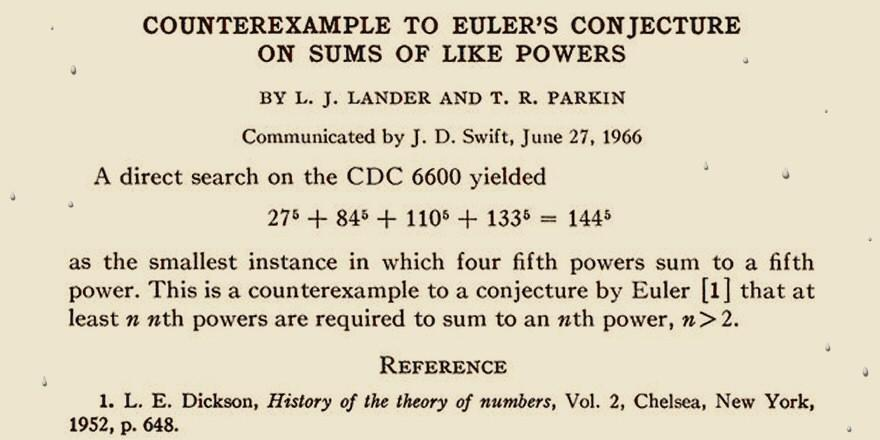
\includegraphics[scale=0.34]{shortest-math-paper.jpg}\end{center}
\end{frame}

\begin{frame}{Proof Logging}
    \vspace*{-1.0em}
    \begin{center}
        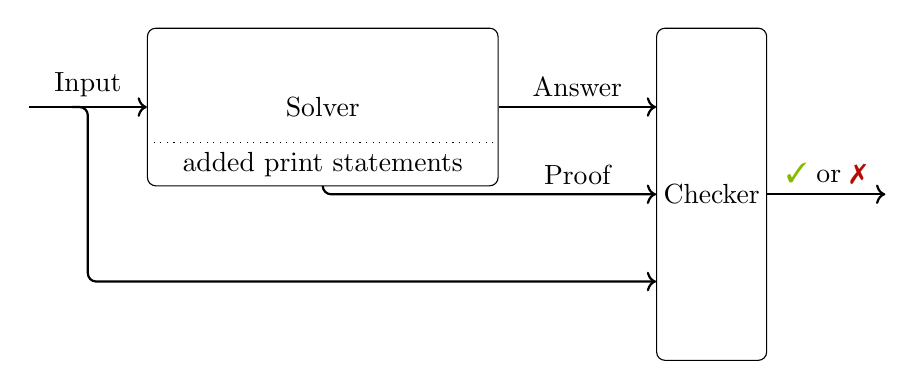
\begin{tikzpicture}
            \node (solver) [inner xsep=5em, inner ysep=2.5em, draw, rounded corners=3pt] { Solver };

            \node (checker) [right=2cm of solver.north east, anchor=north west, inner xsep=0.25em, draw, rounded corners=3pt, minimum height=12em, visible on=<3->] { Checker };

            \node (print) [anchor=south, above=0cm of solver.south, visible on=<2->] { added print statements };
            \draw [dotted, visible on=<2->] (solver.west|-print.north) -- (solver.east|-print.north);

            \draw [->, thick] (solver.east) -- (solver.east -| checker.west)
                coordinate [midway] (solutionmid) node [above, midway] { Answer };

            \draw [->, thick, rounded corners=3pt, visible on=<2->] (solver.south) -- (solver.south |- checker.west)
                -- (checker.west) coordinate [midway] (proofmid);

            \coordinate (prooflabel) at (proofmid-|solutionmid);
            \node [above=0cm of prooflabel, visible on=<2->] { Proof };

            \coordinate [right=1.5cm of checker.east] (verified);
            \draw [->, thick, visible on=<4->] (checker.east) -- (verified) node [above, midway] { \textcolor{uofglawn}{\ding{51}} or \textcolor{uofgpillarbox}{\ding{55}} };

            \coordinate [left=1.5cm of solver.west] (input);
            \draw [->, thick] (input) -- (solver.west) coordinate [midway] (inputmid) node [above, midway] { Input };

            \coordinate (checkerbotleft) at ($(checker.west)+($(checker.west)-(solver.east-|checker.west)$)$);

            \draw [->, thick, rounded corners=3pt, visible on=<3->] ($(inputmid)+(-0.2,0)$) -- (inputmid) -- (inputmid |- checkerbotleft) -- (checkerbotleft);
        \end{tikzpicture}
      \end{center}
    \vspace*{-0.7em}
  \begin{enumerate}
  \item<1->
    Run solver on problem input.
  \item<2->
    Solver also prints out a proof as part of its output.
  \item<3->
    Feed input + solution + proof to proof checker.
  \item<4->
    Verify that proof checker says solution is correct.
  \end{enumerate}
\end{frame}

\begin{frame}{Proof Logging for Boolean Satisfiability}
    \begin{itemize}
        \item A variety of formats for SAT: \ldots, DRAT, FRAT, \ldots.
    \end{itemize}
    \pause
        \centering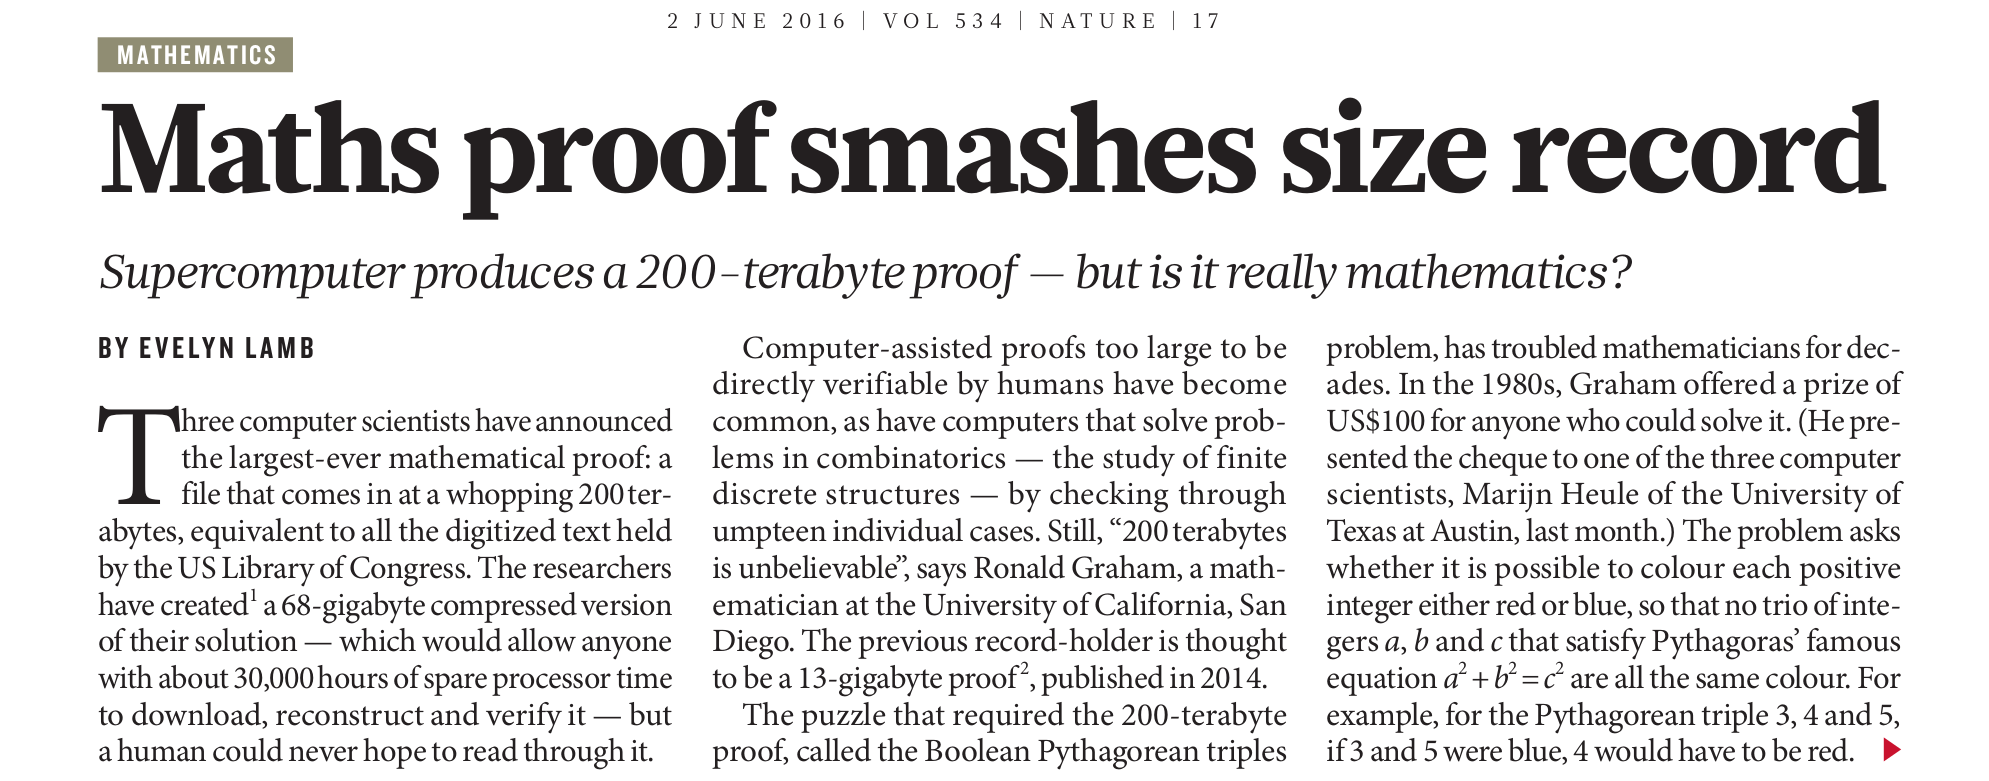
\includegraphics[keepaspectratio=true,scale=0.65]{nature.png}
            \pause
    \begin{itemize}
        \item Until recently: couldn't handle cardinality reasoning, symmetries, \ldots
    \end{itemize}
\end{frame}

\subsection{Bogaerts, Gocht, McCreesh, Nordstr\"om: Certified Dominance and Symmetry Breaking for
Combinatorial Optimisation. JAIR 77 (2023).}

\begin{frame}{The VeriPB Proof System}
    \begin{center}
        \url{https://gitlab.com/MIAOresearch/software/VeriPB}
    \end{center}

    \begin{itemize}
        \item Built upon 0-1 integer linear inequalities: a superset of Boolean CNF.
        \item Provides efficient ways of justifying stronger reasoning, even for
            conventional SAT solvers.
        \item Maybe we can use this for constraint programming too?
    \end{itemize}
\end{frame}

\begin{frame}{Cutting Planes Proofs 1: Linear Inequalities}
    \begin{minipage}[c]{0.35\framewidth}
        \textcolor{uofgcobalt}{\textbf{Model axioms}}
    \end{minipage}\hfill\begin{minipage}[c]{0.60\framewidth}
        \centering From the input
    \end{minipage}\bigskip

    \begin{minipage}[c]{0.35\framewidth}
        \textcolor{uofgcobalt}{\textbf{Addition}}
    \end{minipage}\hfill\begin{minipage}[c]{0.60\framewidth}\begin{prooftree}
        \AxiomC{$\sum_i a_i \ell_i \ge A$}
        \AxiomC{$\sum_i b_i \ell_i \ge B$}
        \BinaryInfC{$\sum_i (a_i + b_i) \ell_i \ge A + B$}
    \end{prooftree}\end{minipage}\bigskip

    \begin{minipage}[c]{0.35\framewidth}
        \textcolor{uofgcobalt}{\textbf{Multiplication}}\\
        for any $c \in \mathbb{N^+}$
    \end{minipage}\hfill\begin{minipage}[c]{0.60\framewidth}\begin{prooftree}
        \AxiomC{$\sum_i a_i \ell_i \ge A$}
        \UnaryInfC{$\sum_i { c a_i \ell_i } \ge c A$}
    \end{prooftree}\end{minipage}
\end{frame}

\begin{frame}{Cutting Planes Proofs 2: 0-1 Variables}
    \begin{minipage}[c]{0.35\framewidth}
        \textcolor{uofgcobalt}{\textbf{Literal axioms}}
    \end{minipage}\hfill\begin{minipage}[c]{0.60\framewidth}\begin{prooftree}
        \AxiomC{~}
        \UnaryInfC{$\ell_i \ge 0$}
    \end{prooftree}\end{minipage}\bigskip

    \begin{minipage}[c]{0.35\framewidth}
        \textcolor{uofgcobalt}{\textbf{Division}}\\
        for any $c \in \mathbb{N^+}$ \\
        assumes normalised form
    \end{minipage}\hfill\begin{minipage}[c]{0.60\framewidth}\begin{prooftree}
        \AxiomC{$\sum_i a_i \ell_i \ge A$}
        \UnaryInfC{$\sum_i {\left\lceil \frac{a_i}{c} \right\rceil} \ell_i \ge \left\lceil \frac{A}{c} \right\rceil$}
    \end{prooftree}\end{minipage}\bigskip

    \begin{minipage}[c]{0.35\framewidth}
        \textcolor{uofgcobalt}{\textbf{Saturation}}\\
        assumes normalised form
    \end{minipage}\hfill\begin{minipage}[c]{0.60\framewidth}\begin{prooftree}
        \AxiomC{$\sum_i a_i \ell_i \ge A$}
        \UnaryInfC{$\sum_i \operatorname{min}\left(a_i, A\right) \ell_i \ge A$}
    \end{prooftree}\end{minipage}
\end{frame}

\begin{frame}{Reverse Unit Propagation (RUP) Proofs}
    \begin{itemize}
        \item Rather than giving explicit derivations, can leave some ``obvious'' facts up
            to the proof checker to work out.
        \item Intuition: can learn a constraint $C$ if the negation of $C$ obviously
            leads to contradiction.
    \end{itemize}
\end{frame}

\begin{frame}{Extended Cutting Planes Proofs}
    We'll also need a way of introducing a new variable that are true if and only if a certain
    constraint holds (\emph{reification}).

    \bigskip

    \begin{minipage}[c]{0.35\framewidth}
        \textcolor{uofgcobalt}{\textbf{Extension}}\\
        $y$ a fresh variable \\
        $C$ any constraint
    \end{minipage}\hfill\begin{minipage}[c]{0.60\framewidth}\begin{prooftree}
        \AxiomC{~}
        \UnaryInfC{$y \Rightarrow C$ \qquad $y \Leftarrow C$}
    \end{prooftree}\end{minipage}

    \bigskip

    In reality: this is a special case of the symmetries and dominance rule.
\end{frame}


\subsection{Gocht, McCreesh, Nordstr\"om: An Auditable Constraint Programming Solver, CP 2022}

\begin{frame}{A Slightly Different Workflow}
    \begin{center}
        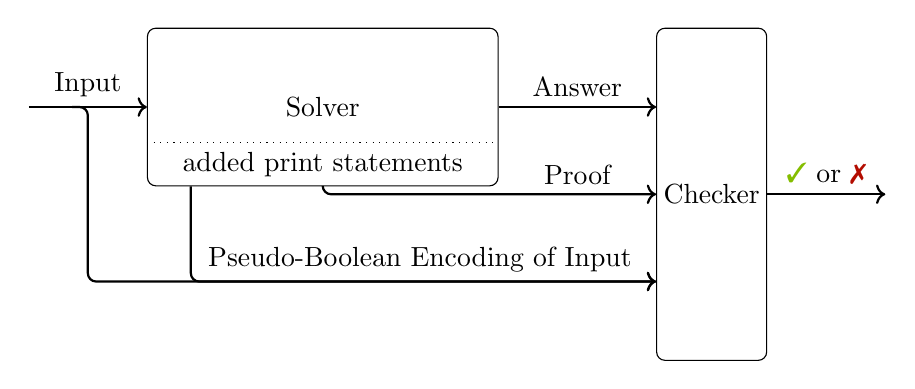
\begin{tikzpicture}
            \node (solver) [inner xsep=5em, inner ysep=2.5em, draw, rounded corners=3pt] { Solver };

            \node (checker) [right=2cm of solver.north east, anchor=north west,
            inner xsep=0.25em, draw, rounded corners=3pt, minimum height=12em, visible on=<3->] { Checker };

            \node (print) [anchor=south, above=0cm of solver.south, visible on=<2->] { added print statements };
            \draw [dotted, visible on=<2->] (solver.west|-print.north) -- (solver.east|-print.north);

            \draw [->, thick] (solver.east) -- (solver.east -| checker.west)
                coordinate [midway] (solutionmid) node [above, midway] { Answer };

            \draw [->, thick, rounded corners=3pt, visible on=<2->] (solver.south) -- (solver.south |- checker.west)
                -- (checker.west) coordinate [midway] (proofmid);

            \coordinate (prooflabel) at (proofmid-|solutionmid);
            \node [above=0cm of prooflabel, visible on=<2->] { Proof };

            \coordinate [right=1.5cm of checker.east] (verified);
            \draw [->, thick, visible on=<5->] (checker.east) -- (verified) node [above, midway] { \textcolor{uofglawn}{\ding{51}} or \textcolor{uofgpillarbox}{\ding{55}} };

            \coordinate [left=1.5cm of solver.west] (input);
            \draw [->, thick] (input) -- (solver.west) coordinate [midway] (inputmid) node [above, midway] { Input };

            \coordinate (checkerbotleft) at ($(checker.west)+($(checker.west)-(solver.east-|checker.west)$)$);

            \draw [->, thick, rounded corners=3pt, visible on=<3>] ($(inputmid)+(-0.2,0)$) --
            (inputmid) -- (inputmid |- checkerbotleft) -- (checkerbotleft) coordinate [midway] (altinputmid);
            \coordinate (solverstart) at ($(solver.south)!0.75!(solver.south west)$);
            \draw [->, thick, rounded corners=3pt, visible on=<4->] (solverstart) -- (solverstart |- checkerbotleft) -- (checkerbotleft);

            \coordinate (encinputlabel) at (altinputmid-|solutionmid);
            \node [above=0cm of encinputlabel, xshift=-2cm, visible on=<4->] { Pseudo-Boolean Encoding of Input };
        \end{tikzpicture}
    \end{center}
\end{frame}

\newcommand{\Redlightning}{\color{uofgthistle}{\Lightning}}

\begin{frame}{Proofs From Search Trees}
    \begin{minipage}[c]{0.45\framewidth}
        \begin{align*}
            2 x_1 + 2 x_2 + 3 x_3 + x_4 + 3 x_5 + 2 x_6 &\le 5 \\
            3 x_1 + 3 x_2 + 4 x_3 + x_4 + 3 x_5 + x_6   &\ge 8
        \end{align*}
        \pause
        \begin{center}
            \tikzstyle{level 1}=[level distance=1.20cm, sibling distance=2.00cm]
            \tikzstyle{level 2}=[level distance=1.20cm, sibling distance=1.00cm]
            \tikzstyle{level 3}=[level distance=1.20cm, sibling distance=0.5cm]
        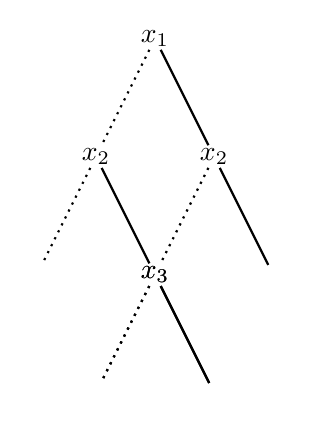
\begin{tikzpicture}
            \node [state] { $x_1$ }
            child {
                node [state] { $x_2$ }
                child {
                    node {\Redlightning}
                    edge from parent [reject]
                }
                child {
                    node [state] { $x_3$ }
                    child {
                        node {\Redlightning}
                        edge from parent [reject]
                    }
                    child {
                        node {\Redlightning}
                        edge from parent [accept]
                    }
                    edge from parent [accept]
                }
                edge from parent [reject]
            }
            child {
                node [state] { $x_2$ }
                child {
                    node [state] { $x_3$ }
                    child {
                        node {\Redlightning}
                        edge from parent [reject]
                    }
                    child {
                        node {\Redlightning}
                        edge from parent [accept]
                    }
                    edge from parent [reject]
                }
                child {
                    node {\Redlightning}
                    edge from parent [accept]
                }
                edge from parent [accept]
            }
            ;
        \end{tikzpicture}
        \end{center}
    \end{minipage}\hfill
    \begin{minipage}[c]{0.45\framewidth}
        \begin{align*}
            \uncover<3->{\operatorname{rup}~ & x_1 + x_2 \ge 1} \\
            \uncover<4->{\operatorname{rup}~ & x_1 + \overline{x}_2 + x_3 \ge 1} \\
            \uncover<5->{\operatorname{rup}~ & x_1 + \overline{x}_2 + \overline{x}_3 \ge 1} \\
            \uncover<6->{\operatorname{rup}~ & x_1 + \overline{x}_2 \ge 1} \\
            \uncover<7->{\operatorname{rup}~ & x_1 \ge 1} \\
            \uncover<8->{\operatorname{rup}~ & \overline{x}_1 + x_2 + x_3 \ge 1} \\
            \uncover<8->{\operatorname{rup}~ & \overline{x}_1 + x_2 + \overline{x}_3 \ge 1} \\
            \uncover<8->{\operatorname{rup}~ & \overline{x}_1 + x_2 \ge 1} \\
            \uncover<8->{\operatorname{rup}~ & \overline{x}_1 \ge 1} \\
            \uncover<9->{\operatorname{rup}~ & 0 \ge 1}
        \end{align*}
    \end{minipage}
\end{frame}

\subsection{Elffers, Gocht, McCreesh, Nordstr\"om: Justifying All Differences Using Pseudo-Boolean Reasoning, AAAI 2020}

\begin{frame}[t]{Justifying All-Different Failures}
%%%
%%% Trying to fine-tune spacing of columns
%%%
  \begin{tabular}%
%%% OLD
%   {r@{\hspace*{0mm}}c@{\hspace*{0.6mm}}c@{\hspace*{0.6mm}}c@{\hspace{0.6mm}}c@{\hspace*{0.6mm}}%
    {r@{\hspace*{0mm}}c@{\hspace*{0.5mm}}c@{\hspace*{0.5mm}}c@{\hspace{0.5mm}}c@{\hspace*{0.5mm}}%
    r@{\hspace*{3mm}}%
%%% OLD
%   r@{\hspace*{0.8mm}}r@{\hspace*{0.8mm}}r@{\hspace*{0.8mm}}r@{\hspace*{0.8mm}}r@{\hspace*{0.8mm}}r@{\hspace*{0.8mm}}r@{\hspace*{0.8mm}}r@{\hspace*{0.8mm}}r@{\hspace*{0.8mm}}%
    r@{\hspace*{0.7mm}}r@{\hspace*{0.7mm}}r@{\hspace*{0.7mm}}r@{\hspace*{0.7mm}}r@{\hspace*{0.7mm}}r@{\hspace*{0.7mm}}r@{\hspace*{0.7mm}}r@{\hspace*{0.7mm}}r@{\hspace*{0.7mm}}%
    ll}
    $V \in \{$
    &
      $1$
    &
    &
    &
      $4$ \hspace*{1.2mm} $5$
    &
      $\}$
    & \phantom{$-v_{{=}1}$}
    &
    & \phantom{$-w_{{=}1}$}
    &
    & \phantom{$-x_{{=}1}$}
    &
    & \phantom{$-y_{{=}1}$}
    &
    & \phantom{$-z_{{=}1}$}
    &
    \\

    $\alertblue<2->{W}
%         \only<2->{{\color{uofgcobalt}W}}
    \in \{$
    &
      \alertred<3>{$1$}
    &
      \alertred<3>{$2$}
    &
      \alertred<3>{$3$}
    &
    &
      $\}$
    &
      $
      \only<1-2>{\phantom{w_{{=}1}}}\only<3->{\alertred<3>{w_{{=}1}}}
      $
    &
      $\only<1-2>{\phantom{+}}\only<3->{\alertred<3>{+}}$
    &
      $\only<1-2>{\phantom{w_{{=}2}}}\only<3->{\alertred<3>{w_{{=}2}}}$
    &
      $\only<1-2>{\phantom{+}}\only<3->{\alertred<3>{+}}$
    &
      $\only<1-2>{\phantom{w_{{=}3}}}\only<3->{\alertred<3>{w_{{=}3}}}$
    &
    &
    &
    &
    &
      $\only<1-2>{\phantom{ \ge \phantom{-}1}}\only<3->{\alertred<3>{ \ge\phantom{-} 1}}$
    &
      \uncover<3->{$[$
      $W\!$ takes some value
      $\!]$}
    \\
    $\alertblue<2->{X} \in \{$
    &
%           $\only<1>{X}\only<2->{{\color{uofgcobalt}X}} \in \{$ &
    &
      $2$
    &
      $3$
    &
    &
      $\}$ &
    &
    &
      $\only<1-3>{\phantom{x_{{=}2}}}\only<4->{x_{{=}2}}$
    &
      $\only<1-3>{\phantom{+}}\only<4->{+}$
    &
      $\only<1-3>{\phantom{x_{{=}3}}}\only<4->{x_{{=}3}}$
    &
    &
    &
    &
    &
      $\only<1-3>{\phantom{ \ge\phantom{-} 1}}\only<4->{ \ge\phantom{-} 1}$
    &
      \uncover<4->{$[$
      $X$ takes some value
      $\!\!\:]$}
    \\
    % $\only<1>{Y}\only<2->{{\color{uofgcobalt}Y}} \in \{$
    $\alertblue<2->{Y} \in \{$
    &
      $1$
    &
    &
      $3$
    &
    &
      $\}$
    &
      $\only<1-3>{\phantom{y_{{=}1}}}\only<4->{y_{{=}1}}$
    &
    &
    &
      $\only<1-3>{\phantom{+}}\only<4->{+}$
    &
      $\only<1-3>{\phantom{y_{{=}3}}}\only<4->{y_{{=}3}}$
    &
    &
    &
    &
    &
      $\only<1-3>{\phantom{ \ge\phantom{-} 1}}\only<4->{ \ge\phantom{-} 1}$
    &
      \uncover<4->{$[$
      $Y$ takes some value
      $]$}
    \\
    % $\only<1>{Z}\only<2->{{\color{uofgcobalt}Z}} \in \{$
    $\alertblue<2->{Z} \in \{$
    &
      $1$
    &
    &
      $3$
    &
    &
      $\}$
    &
      $\only<1-3>{\phantom{z_{{=}1}}}\only<4->{z_{{=}1}}$
    &
    &
    &
      $\only<1-3>{\phantom{+}}\only<4->{+}$
    &
      $\only<1-3>{\phantom{z_{{=}3}}}\only<4->{z_{{=}3}}$
    &
    &
    &
    &
    &
      $\only<1-3>{\phantom{ \ge\phantom{-} 1}}\only<4->{ \ge\phantom{-} 1}$
    &
      \uncover<4->{$[$
      $Z$ takes some value
      $]$}
    \\[0.5cm]

    \only<5->{
    &
      $\rightarrow$
    &
    &
    &
    &
    &
      $-v_{{=}1}$
    &
      $+$
    &
      $-w_{{=}1}$
    &
      $+$
    &
    &
    &
      $-y_{{=}1}$
    &
      $+$
    &
      $-z_{{=}1}$
    &
      $ \ge -1$
    &
      \uncover<5->{$[$
      At most  one variable
      $=1$
      $]$}
    \\

    &
    &
      $\rightarrow$
    &
    &
    &
    &
    &
    &
      $-w_{{=}2}$
    &
      $+$
    &
      $-x_{{=}2}$
    &
    &
    &
    &
    &
      $ \ge -1$
    &
      \uncover<5->{$[$
      At most  one variable
      $=2$
      $]$}
    \\

    &
    &
    &
      $\rightarrow$
    &
    &
    &
    &
    &
      $-w_{{=}3}$
    &
      $+$
    &
      $-x_{{=}3}$
    &
      $+$
    &
      $-y_{{=}3}$
    &
      $+$
    &
      $-z_{{=}3}$
    &
    $ \ge -1$
    &
      \uncover<5->{$[$
      At most  one variable
      $=3$
      $]$}
    \\[0.5cm]
}
\only<6->{
    &
    &
    &
    &
    &
    &
      $-v_{{=}1}$
    &
    &
    &
    &
    &
    &
    &
    &
    &
      $ \ge \phantom{-}1$
    &
      \uncover<5->{$[$
      Sum all constraints so far
      $]$}
    \\
    }
\only<7->{
    &
    &
    &
    &
    &
    &
      $ v_{{=}1}$
    &
    &
    &
    &
    &
    &
    &
    &
    &
      $ \ge \phantom{-}0$
    &
      \uncover<5->{$[$
      Variable $ v_{{=}1}$ non-negative
      $]$}
    \\[0.5cm]
}
\only<8->{
    &
    &
    &
    &
    &
    &
      $0$
    &
    &
    &
    &
    &
    &
    &
    &
    &
      $ \ge \phantom{-}1$
    &
      \uncover<5->{$[$
      Sum above two constraints
      $]$}
    \\
}
    &
    $\phantom{\rightarrow}$ &
    $\phantom{\rightarrow}$ &
    $\phantom{\rightarrow}$ &
    &
    &
    $\phantom{-v_{{=}1}}$ &
    $\phantom{+}$ &
    $\phantom{-w_{{=}1}}$ &
    $\phantom{+}$ &
    $\phantom{-y_{{=}1}}$ &
    $\phantom{+}$ &
    $\phantom{-y_{{=}1}}$ &
    $\phantom{+}$ &
    $\phantom{-z_{{=}1}}$ &
    $\phantom{ \ge -1}$ \\
    \end{tabular}
\end{frame}

\begin{frame}{This Actually Works!}
    \begin{center}
        \url{https://github.com/ciaranm/glasgow-constraint-solver}
    \end{center}
    \bigskip
    \begin{itemize}
        \item MIT licence, written in fancy modern C++.
        \item All-different, integer linear inequality (including for variables
            with very large domains), smart table, minimum / maximum of an array,
            element, absolute value, knapsack, regular expression,
            Hamiltonian circuit.
    \end{itemize}
\end{frame}

\section{Symmetry Constraints}

\begin{frame}{Symmetries}
    \begin{center}
    \begin{minipage}{8cm}
        \centering
        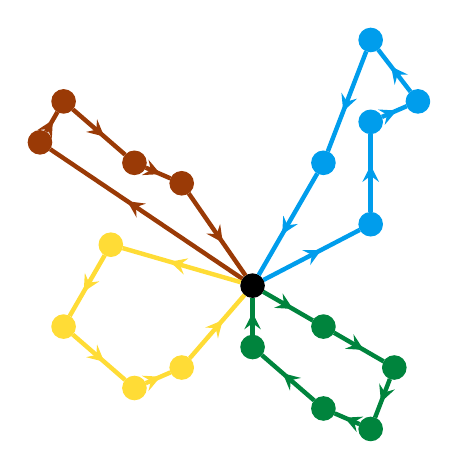
\begin{tikzpicture}
        \begin{scope}[yscale=2.6, xscale=3.0]
        \node (depot) [inner sep=3pt, draw, fill, circle] at (0,0) {};

        \node (RC1) [inner sep=3pt, draw, fill, circle, color=uofgcobalt] at (0.5,0.3) {};
        \node (RC2) [inner sep=3pt, draw, fill, circle, color=uofgcobalt] at (0.5,0.8) {};
        \node (RC3) [inner sep=3pt, draw, fill, circle, color=uofgcobalt] at (0.7,0.9) {};
        \node (RC4) [inner sep=3pt, draw, fill, circle, color=uofgcobalt] at (0.5,1.2) {};
        \node (RC5) [inner sep=3pt, draw, fill, circle, color=uofgcobalt] at (0.3,0.6) {};

        \begin{scope}[decoration={markings, mark=at position 0.6 with {\arrow{stealth}}}]
            \draw [postaction={decorate}, ultra thick, color=uofgcobalt] (depot) -- (RC1);
            \draw [postaction={decorate}, ultra thick, color=uofgcobalt] (RC1)   -- (RC2);
            \draw [postaction={decorate}, ultra thick, color=uofgcobalt] (RC2)   -- (RC3);
            \draw [postaction={decorate}, ultra thick, color=uofgcobalt] (RC3)   -- (RC4);
            \draw [postaction={decorate}, ultra thick, color=uofgcobalt] (RC4)   -- (RC5);
            \draw [postaction={decorate}, ultra thick, color=uofgcobalt] (RC5)   -- (depot);
        \end{scope}

        \node (RR1) [inner sep=3pt, draw, fill, circle, color=uofgrust] at (-0.9,0.7) {};
        \node (RR2) [inner sep=3pt, draw, fill, circle, color=uofgrust] at (-0.8,0.9) {};
        \node (RR3) [inner sep=3pt, draw, fill, circle, color=uofgrust] at (-0.5,0.6) {};
        \node (RR4) [inner sep=3pt, draw, fill, circle, color=uofgrust] at (-0.3,0.5) {};

        \begin{scope}[decoration={markings, mark=at position 0.6 with {\arrow{stealth}}}]
            \draw [postaction={decorate}, ultra thick, color=uofgrust] (depot) -- (RR1);
            \draw [postaction={decorate}, ultra thick, color=uofgrust] (RR1)   -- (RR2);
            \draw [postaction={decorate}, ultra thick, color=uofgrust] (RR2)   -- (RR3);
            \draw [postaction={decorate}, ultra thick, color=uofgrust] (RR3)   -- (RR4);
            \draw [postaction={decorate}, ultra thick, color=uofgrust] (RR4)   -- (depot);
        \end{scope}

        \node (RS1) [inner sep=3pt, draw, fill, circle, color=uofgsunshine] at (-0.6,0.2) {};
        \node (RS2) [inner sep=3pt, draw, fill, circle, color=uofgsunshine] at (-0.8,-0.2) {};
        \node (RS3) [inner sep=3pt, draw, fill, circle, color=uofgsunshine] at (-0.5,-0.5) {};
        \node (RS4) [inner sep=3pt, draw, fill, circle, color=uofgsunshine] at (-0.3,-0.4) {};

        \begin{scope}[decoration={markings, mark=at position 0.6 with {\arrow{stealth}}}]
            \draw [postaction={decorate}, ultra thick, color=uofgsunshine] (depot) -- (RS1);
            \draw [postaction={decorate}, ultra thick, color=uofgsunshine] (RS1)   -- (RS2);
            \draw [postaction={decorate}, ultra thick, color=uofgsunshine] (RS2)   -- (RS3);
            \draw [postaction={decorate}, ultra thick, color=uofgsunshine] (RS3)   -- (RS4);
            \draw [postaction={decorate}, ultra thick, color=uofgsunshine] (RS4)   -- (depot);
        \end{scope}

        \node (RL1) [inner sep=3pt, draw, fill, circle, color=uofgleaf] at (0.3,-0.2) {};
        \node (RL2) [inner sep=3pt, draw, fill, circle, color=uofgleaf] at (0.6,-0.4) {};
        \node (RL3) [inner sep=3pt, draw, fill, circle, color=uofgleaf] at (0.5,-0.7) {};
        \node (RL4) [inner sep=3pt, draw, fill, circle, color=uofgleaf] at (0.3,-0.6) {};
        \node (RL5) [inner sep=3pt, draw, fill, circle, color=uofgleaf] at (0,-0.3) {};

        \begin{scope}[decoration={markings, mark=at position 0.6 with {\arrow{stealth}}}]
            \draw [postaction={decorate}, ultra thick, color=uofgleaf] (depot) -- (RL1);
            \draw [postaction={decorate}, ultra thick, color=uofgleaf] (RL1)   -- (RL2);
            \draw [postaction={decorate}, ultra thick, color=uofgleaf] (RL2)   -- (RL3);
            \draw [postaction={decorate}, ultra thick, color=uofgleaf] (RL3)   -- (RL4);
            \draw [postaction={decorate}, ultra thick, color=uofgleaf] (RL4)   -- (RL5);
            \draw [postaction={decorate}, ultra thick, color=uofgleaf] (RL5)   -- (depot);
        \end{scope}
        \end{scope}
    \end{tikzpicture}
\end{minipage}\begin{minipage}{12cm}
    \truck{uofgrust} \drivera\driverb\raisebox{1mm}{:} \bed\parcel\chair\parcel

    \medskip

    \truck{uofgcobalt} \driverb\drivera\raisebox{1mm}{:}
    \chair\trashpanda\parcel\parcel\present


    \medskip

    \truck{uofgsunshine} \driverb\driverb\raisebox{1mm}{:} \tree\parcel\chair\present

    \medskip

    \truck{uofgleaf} \drivera\phantom{\drivera}\raisebox{1mm}{:}
    \parcel\parcel\laptop\parcel\parcel

    \bigskip

    \begin{itemize}
        \item<2-> $\operatorname{routes}(\raisebox{-2pt}{\truck{uofgrust}}, 0) < \operatorname{routes}(\raisebox{-2pt}{\truck{uofgcobalt}}, 0)$
        \item<3-> $\operatorname{routes}(\raisebox{-2pt}{\truck{uofgcobalt}}, 0) < \operatorname{routes}(\raisebox{-2pt}{\truck{uofgsunshine}}, 0)$
        \item<4-> $\operatorname{routes}(\raisebox{-2pt}{\truck{uofgsunshine}}, 0) < \operatorname{routes}(\raisebox{-2pt}{\truck{uofgleaf}}, 0)$ \only<5->{Maybe?}
        \item<6-> $\operatorname{vehicle}(\raisebox{-2pt}{\drivera}) < \operatorname{vehicle}(\raisebox{-2pt}{\driverb})$ etc\ldots
        \item<7-> $\operatorname{routes}(\raisebox{-2pt}{\truck{uofgrust}}, 0) < \operatorname{routes}(\raisebox{-2pt}{\truck{uofgrust}}, 1)$ \only<8->{Sus.}
    \end{itemize}
\end{minipage}
\end{center}
\end{frame}

\begin{frame}{Symmetries and Proofs}
    \begin{itemize}
        \item Could just put the symmetry elimination constraints in the definition, and then log
            their propagations.
        \item<2-> But modellers often get these constraints wrong.
            \begin{itemize}
                \item<2-> This checks that the solver propagates less-than correctly, not that the
                    less-thans are valid.
            \end{itemize}
        \item<3-> Alternative idea: introduce these constraints inside the proof, which is only
            possible if they're valid.
        \item<4-> Not possible in raw cutting planes: constraints aren't implied, but rather use
            \emph{without loss of satisfaction} or \emph{without loss of optimality} reasoning.
    \end{itemize}
\end{frame}

\begin{frame}{Reasoning Without Loss of Satisfaction}
    \begin{itemize}
        \item Allowed to introduce a new constraint $C$ into a decision problem $P$ if for all solutions $\rho$, either
            \begin{itemize}
                \item $\rho$ satisfies $C$, or
                \item We can provide an efficiently-verifiable way of fixing $\rho$ to satisfy $C$.
            \end{itemize}
        \item So, only need to care about solutions that satisfy $P$ but not $C$.
    \end{itemize}
\end{frame}

\begin{frame}{Reasoning Without Loss of Optimality}
    \begin{itemize}
        \item What about optimisation problems?
        \item Also need to show that fixing $\rho$ does not worsen the objective.
        \item <2-> In fact, if fixing strictly improves the objective, we do not even need the fixed
            solution to satisfy $C$.
        \item <3-> Final trick: we can invent our own objective function for decision problems, or
            extend the objective for optimisation problems.
        \item <3-> Of all the (optimal?) solutions to the problem you care about, I'm going to find
            you the one that minimises the symmetry ordering.
    \end{itemize}
\end{frame}

\section{Conclusion}

\begin{frame}{Conclusion}
    \begin{itemize}
        \item Trust solutions, not solvers.
        \item Can store an auditable record of what problem was solved, and how its solution
            was reached.
        \item Can help reduce modelling errors too.
        \item Proof logging useful for other things too:
            \begin{itemize}
                \item Speeds up solver development.
                \item Can analyse proofs to design better solvers.
                \item Explainability?
            \end{itemize}
    \end{itemize}
\end{frame}

{
    \usebackgroundtemplate{
        \tikz[overlay, remember picture]
        \node[at=(current page.south), anchor=south, yshift=-1cm, inner sep=0pt]{\includegraphics[keepaspectratio=true, width=\paperwidth]{../../images/background2.jpg}};
    }

    \begin{frame}[plain,noframenumbering]
        \begin{tikzpicture}[remember picture, overlay]
            \node at (current page.north west) {
                \begin{tikzpicture}[remember picture, overlay]
                    \fill [fill=uofguniversityblue, anchor=north west] (0, 0) rectangle (\paperwidth, -2.8cm);
                \end{tikzpicture}
            };

            \node (logo) [anchor=north east, shift={(-0.8cm,-0.2cm)}] at (current page.north east) {
                
\includegraphics[keepaspectratio=true,scale=0.5]{../../images/UoG_keyline.pdf}
            };

            \node (logo2) [anchor=north, below=0.2cm of logo.south] {
                
\includegraphics[keepaspectratio=true,scale=0.1]{../../images/RAEngWhite.pdf}
            };

            \coordinate (logos) at ($(logo.south)!0.5!(logo2.north)$);

            \node [anchor=west, xshift=0.8cm] at (current page.west |- logos) {
                \begin{minipage}{0.60\paperwidth}\raggedright
                    \textcolor{white}{\url{https://ciaranm.github.io/}} \\[0.3cm]
                    \textcolor{white}{\href{mailto:ciaran.mccreesh@glasgow.ac.uk}{\nolinkurl{ciaran.mccreesh@glasgow.ac.uk}}}
                \end{minipage}
            };
        \end{tikzpicture}
    \end{frame}
}

\end{document}

